\section{Tests and Results}
\label{sec:tests}

\subsection{Setup}
\label{sec:setup}

\emph{Data.} PKU37~\cite{geng2022triplet} provides 37 cross sections of $640 \times 640$ pixels from a
spectral domain scanner, references averaged over 50 frames, split by clean image identity into 27, 5
and 5 for training, validation and testing, giving 1388, 173 and 173 pairs, and is the only training
domain. Duke17~\cite{fang2012sparsity} provides 17 paired B scans of $970 \times 520$ from a clinical
scanner at another institution, of which we use the 16 stored under the naming the released loader
reads, and Duke2013~\cite{fang2013fast} the 18 volumes of $900 \times 450$ of its test split.

\emph{Transfer protocol.} Every model is trained once on PKU37 and applied to the Duke sets directly,
with nothing fitted, recalibrated or selected on Duke data beyond the per image quantity the gate of
Equation~\eqref{eq:gate} computes by the same rule as on PKU37. The original submission instead
adapted the wrapper for fifteen further epochs on the other subjects of the target set, leave one
subject out, backbone frozen, with an L2 penalty holding every trainable weight near its PKU37 value,
and we rerun that for NAFNet in the adapted block of Table~\ref{tab:pku37}, with per subject spreads
in the supplementary file.

\emph{Measures.} Peak signal to noise ratio against the clean reference measures fidelity. Six
clinical measures, given as percentage change from backbone to corrected output, are contrast to
noise ratio for tissue against background, tissue contrast index for dynamic range in tissue, edge
preservation index for agreement with the reference edge map, boundary sharpness for the gradient
across layer boundaries, equivalent number of looks for speckle suppression, and signal to noise
ratio against the noise floor. Each is computed per image then averaged, never pooled across a batch,
since pooling inflates the result. 

\begin{table*}[!tb]
\centering
\caption{PKU37 test set of 173 images, then Duke17 and Duke2013 with no adaptation, then the adapted
protocol of the original submission for NAFNet described in Section~\ref{sec:setup}. Columns give the
backbone peak signal to noise ratio in decibels, its change after correction with the spread across
three seeds, and the six clinical measures as percentage change from backbone output to corrected
output, bold where the mean exceeds the seed spread. The adapted rows come from one seed and one fold
per subject, so they carry no spread and no bold. The two lowest blocks use the selected NAFNet checkpoint on the
same 173 test images with one component removed or an alternative operator substituted. Full spreads
are in the supplementary file.}
\label{tab:pku37}
\setlength{\tabcolsep}{4pt}
\footnotesize
\begin{tabular}{lccccccc}
\toprule
Backbone & $\Delta$PSNR & $\Delta$CNR & $\Delta$TCI & $\Delta$EPI & $\Delta$BS & $\Delta$ENL & $\Delta$SNR \\
\midrule
NAFNet & -0.18 & $\mathbf{+3.49}$ & $\mathbf{+1.91}$ & $\mathbf{+1.20}$ & $\mathbf{+3.89}$ & $\mathbf{+23.74}$ & $\mathbf{+11.10}$ \\
DnCNN & -0.98 & $\mathbf{+11.30}$ & +0.99 & $\mathbf{+4.14}$ & -1.44 & $\mathbf{+57.14}$ & $\mathbf{+22.95}$ \\
SwinIR & -0.17 & $\mathbf{+7.33}$ & $\mathbf{+11.45}$ & $\mathbf{+2.68}$ & $\mathbf{+1.82}$ & $\mathbf{+28.32}$ & $\mathbf{+11.54}$ \\
KBNet & -0.90 & $\mathbf{+6.93}$ & $\mathbf{+5.92}$ & +0.00 & $\mathbf{+2.58}$ & $\mathbf{+25.30}$ & $\mathbf{+7.95}$ \\
\bottomrule
\end{tabular}

\end{table*}

\subsection{In distribution results}
\label{sec:results_id}
Table~\ref{tab:pku37} reports the PKU37 test set and Fig.~\ref{fig:subjective_pku37} the visual
comparison across the four backbones. Contrast rose on 2064 of the 2076 image and seed combinations.
The twelve exceptions all belong to NAFNet, the backbone with the smallest mean contrast gain, fall on
ten images whose backbone PSNR lies above the NAFNet mean, and none exceeds 0.4 percent. The gain was
larger where the backbone PSNR was lower, with a per image Spearman correlation between minus 0.46 and
minus 0.71 across the four backbones. Of the 24 backbone by measure pairs, 21 are positive by more
than one seed spread, one is positive but inside it, the tissue contrast index of DnCNN, one is
unchanged at 0.00 percent, the edge preservation of KBNet, and one falls, the boundary sharpness of
DnCNN at minus 1.44 percent. The fidelity cost ranges from 0.17 dB on SwinIR to 0.98 dB on DnCNN, and
the two backbones that pay least are the two whose six measures all rise.

\begin{figure*}[!tb]
\centering
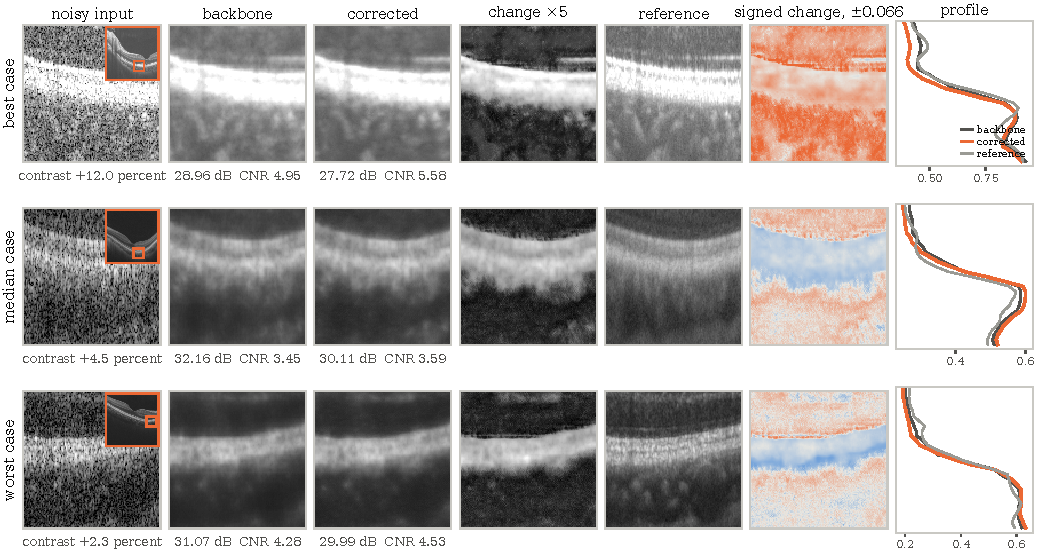
\includegraphics[width=0.9\textwidth]{figures/fig_subjective_pku37.pdf}
\caption{Visual comparison on the PKU37 test image of median backbone fidelity, one row per backbone,
in the 56 by 136 pixel band marked on the thumbnail where the NAFNet correction was largest. The
eight gray cells share one display range, set to the values they contain so that nothing is clipped,
and the signed difference uses a fixed scale of plus or minus 0.06. The mean absolute change is about
one percent of the intensity range, most for SwinIR and least for KBNet, from the seed 0 checkpoints
of Table~\ref{tab:pku37}. The scatter places this image, ringed, among all 173 test images at three
seeds for four backbones, with the twelve NAFNet points below zero marked. Full resolution pairs for
every backbone are in the supplementary file.}
\label{fig:subjective_pku37}
\end{figure*}

\subsection{Transfer to other scanners}
\label{sec:results_ood}
Table~\ref{tab:pku37} reports the no adaptation protocol on Duke17 and Duke2013. All six clinical
measures are positive on both target sets for NAFNet and SwinIR, the fidelity cost stays inside
0.35 dB for those two, and 40 of the 48 backbone by measure by set pairs are positive, the eight
exceptions being the tissue contrast index and the boundary sharpness of DnCNN and the edge
preservation and the signal to noise ratio of KBNet. Contrast rises on every backbone and both sets.

Adaptation, the last block, raises contrast on both scanners, from $+7.5$ to $+10.7$ percent on
Duke17 and from $+7.4$ to $+15.4$ on Duke2013, where it also lifts the tissue contrast index from
$+1.4$ to $+5.1$. It pays on both, a further 0.06 and 0.10 dB of fidelity and a signal to noise ratio
that falls from $+5.4$ to $+2.9$ percent on Duke17 and from $+9.3$ to $-5.3$ on Duke2013, down on 15
of 18 subjects, while the other measures move in opposite directions on the two sets. The only
measure adaptation reliably improves is the one the frozen model already improves, so the frozen
model is the one we recommend and use everywhere else.

\subsection{Contribution of each clinical property}
\label{sec:predicate_ablation}
One property at a time is switched off
at test time, by setting its score to the satisfied value and its failure map to zero, and the whole
test set is re evaluated. Only $P_5$, $P_1$ and $P_2$ move any measure by more than a quarter point.
$P_5$ costs the most at 3.19 points of the speckle gain, $P_1$ 1.72 and $P_2$ 0.74, while $P_3$,
$P_4$ and $P_6$ change nothing by more than 0.23 points. We keep all six, because they are the vocabulary of the rule layer and of the explanation shown to the
reader, and one that rarely fires here can fire on another scanner.

\subsection{Sensitivity to the rule constants}
\label{sec:sensitivity}
The rule layer contains a base level, five rule weights and five budgets. The budgets are tied by the identity of Section~\ref{sec:allocation_defect}, so they are held. We
vary the base level and the two
rule weights that carry the allocation, and we replace the Lukasiewicz conjunction by the product and
by the minimum, the two other standard choices, to test whether the specific logic matters. No
variation turns any of the six clinical measures negative. Across the fourteen variations the
contrast gain lies between 3.5 and 4.5 percent, the tissue contrast index between 2.3 and 2.9
percent, the speckle measure between 22.6 and 23.5 percent and the fidelity cost between 0.16 and
0.23 dB. The base level is the only constant whose effect is visible, since lowering it raises
contrast and costs fidelity together, while the two rule weights move the result by under a fifth of
a point. The product and the minimum change the contrast gain from 3.7 to 3.5 percent and leave the
other five measures within one part in fifty, so the result rests on the shape of the rule layer and
not on the particular conjunction. No setting of either gate rule of
Section~\ref{sec:weight_selection} recovers boundary sharpness on DnCNN.

\subsection{Contribution of each component}
\label{sec:component_ablation}
The component block of Table~\ref{tab:pku37} removes one component at a time. Replacing the rule layer by a uniform
allocation cuts the contrast gain from 3.7 to 0.8 percent and the tissue contrast index from 2.4 to
0.4 percent while doubling the fidelity cost, the clearest evidence that the allocation and not the
capacity of the correctors produces the clinical gain. Removing the edge branch turns both measures
negative, and removing the cooperation map costs about a third of the contrast gain. Removing
background smoothing leaves contrast, edge preservation and boundary sharpness almost intact while
the speckle measure collapses from 23.3 to 5.8 percent and the signal to noise ratio from 10.7 to 2.9
percent.

\subsection{Comparison at matched complexity}
\label{sec:matched}
Three alternatives act on the same frozen backbone output. The first is the same architecture, budget,
objective and ten epochs, with the rule layer replaced by a uniform allocation for the whole of
training rather than only at test time, keeping the properties and the safety layer. It was fitted
before the gate search, so it carries the percentile gate rather than the tissue bounded gate NAFNet
was finally selected with. The other two are classical operators, unsharp masking and contrast limited
adaptive histogram equalisation, tuned on the validation split. Uniform allocation reaches a larger
contrast gain and a much larger tissue contrast index than the full method, for 0.42 dB against 0.17
dB, and is worse on four of the six measures, so the two are not ordered. What the full method buys
with its fidelity is the per pixel account of why each change was made. The classical operators give
the largest contrast numbers and fail elsewhere, lowering edge preservation by about 3.5 percent and
the speckle measure by about 36 percent while raising boundary sharpness by about 25 percent by
sharpening noise with structure, with adaptive equalisation also costing 4.4 dB.


\subsection{Does the cooperation map predict error}
\label{sec:confidence_check}
Called a confidence map in the original submission, this component was tested against the absolute
error of the backbone output over \NImages{} images, and it does not predict that error. The rank
correlation is \CalibRho{}, so the map is ordered the wrong way rather than merely uninformative, and
removing the pixels it ranks as least reliable raises the remaining error to 1.88 times the starting
value where an oracle ranking reaches 0.07, a sparsification error of \CalibAuse{}. The map is
nevertheless load bearing, since replacing it by a constant lowers the contrast gain from $+3.71$ to
$+2.51$ percent and worsens five of the six clinical measures. Nothing in the objective shows the head the error of the backbone, so we call it a cooperation map
rather than a confidence.

\subsection{Do the theoretical conditions hold on real data}
\label{sec:theory_check}
We perturb the rule truth values and compare the ratio of Equation~\eqref{eq:stability_def} with the
constant of Equation~\eqref{eq:lipschitz}, and we measure the tissue gain, the background leakage and
the ratio of background standard deviations on every image against the hypotheses of
Theorem~\ref{thm:cnr}. The stability bound holds with room to spare, a constant of \LipTheory{} from
Equation~\eqref{eq:lipschitz} against a largest measured ratio of \LipMeasured{} over \NImages{}
images, so the proof is conservative rather than tight. The
allocation map spans \AllocMin{} to \AllocMax{} with mean \AllocMean{} and standard deviation
\AllocStd{}, and \AllocClamp{} percent of pixels sit at either end of its clamp, direct evidence that
the rule layer does work after the repair of Section~\ref{sec:allocation_defect}.

The margin condition holds on
\CondMargin{} of \NImages{} images and the standard deviation ratio condition on \CondSigma{}, a bare
majority, with mean ratio \SigmaRatio{} below one, which is why the result holds in the mean. Where a
hypothesis fails the theorem predicts nothing, and the measured contrast change there does not differ
systematically in sign, so the conditions are sufficient and not necessary. Both leakage terms of
Theorem~\ref{thm:cnr} sit far below the mean absolute change over the whole image, \GlobalChange{}, at
\EtaT{} in tissue and \EtaB{} in background, with means near zero and a long negative tail, so the per
image sign carries what the theorem needs. Tissue is positive on \EtaTPos{} of \NImages{} images and
background negative on \EtaBNeg{}, the direction the decomposition assumes.

\subsection{Safety, and whether the correction invents structure}
\label{sec:safety_check}
A correction that raises contrast could sharpen a boundary that is not there or erase a faint one
that is, and the clean reference lets us measure both. Two measures move against it. An edge appears where the
reference has none on \EdgeInvCorr{} percent of pixels after correction against \EdgeInvBack{} percent
for the backbone output, a rise on \EdgeInvUp{} of \NImages{} images with $p = 1.9 \times 10^{-12}$ under a two
sided Wilcoxon signed rank test on the paired per image values, and the retention of structures whose
reference contrast falls in the lowest decile falls from \WeakRetBack{} to \WeakRetCorr{} percent, on
\WeakRetDown{} of \NImages{} images with $p = 6.2 \times 10^{-30}$. Both are small, 0.03 points of invented
edge rate and 2.9 points of retention, neither is zero by construction, since the clamp of
Section~\ref{sec:safety} bounds how far a pixel may move and not how many cross an edge threshold, and
Section~\ref{sec:discussion} lists both as limitations. What separates the correction from a
sharpening filter is Section~\ref{sec:matched}, where the classical sharpeners lose edge preservation
and the speckle measure while the wrapper gains on both. The two
layer boundaries a clinician reads are not displaced, with a mean absolute shift of \IlmShiftBack{} to
\IlmShiftCorr{} pixels for the inner limiting membrane, an improvement, and \RpeShiftBack{} to
\RpeShiftCorr{} for the retinal pigment epithelium, unchanged within the spread across images. Dark
fluid like regions occupy \DarkFrac{} percent of the image area with a mean absolute change of
\DarkChange{} inside them against \GlobalChange{} over the whole image, and the largest change on any
single image anywhere in the test set is \GlobalMax{}, so the correction is quieter
where a dark region carries the finding. Boundary sharpness is not worsened on \BoundOK{} of
\NImages{} images, a count, since the per image worst case is what matters for trusting a scan. Of the three constraints of
Section~\ref{sec:safety}, energy holds on \ConEnergy{} of \NImages{} images and bounded change on
\ConLip{}, and only the no sacrifice constraint ever fails, on \NImages{} minus \ConPareto{} of them. Acceptance needs two of three and no image falls
below two, so the blend of Equation~\eqref{eq:blend} returns the candidate in full everywhere and the
safety layer never had to act here.

\subsection{Cost of moving to a new backbone}
\label{sec:transfer_cost}
A new backbone means refitting the whole wrapper, not only the head that reads its features. The
trainable count is \num{168630} shared parameters plus a head whose width follows the feature tensor it
reads, \num{175893} in all for NAFNet and \num{254538} for SwinIR, against about seven million in the
backbone, an increase of about 2.4 percent.
Every backbone is fitted on the same 1388 PKU37 pairs for the same ten epochs, so only the wall clock
time and the spread across seeds vary. Fitting one seed of the selected setting on a single RTX 5070
Ti takes 2.0 minutes for NAFNet, 2.5 for KBNet, 3.9 for DnCNN and 8.3 for SwinIR, an ordering that
follows the cost of one backbone forward pass. The spread of the
fidelity cost across the three seeds is 0.02 dB for NAFNet, 0.06 for SwinIR, 0.08 for KBNet and 0.21
for DnCNN. The backbone with the widest spread is also the only one with a clinical measure that
falls, so a new user should read the seed spread as the first warning sign rather than the mean.














